\section{Théorie des probabilités}

Modern probability is the théorie de la mesure with one extra axiom: the total mass
is one. Everything in this chapter is a specialisation of chapters 2 and 3 --- a
probability is a mesure, a variable aléatoire is a mesurable function, an espérance
is an intégrale de Lebesgue --- and the work is in learning what the specialisation
buys. What it buys is a vocabulary that the general theory does not have: lois,
fonctions de répartition, densités, indépendance, moments, and the three
inequalities that every limit theorem in chapter 8 rests on.\\

Les résultats présentés généralisent ceux vus au chapitre 1 dans le cas des
probabilités discrètes. Certaines preuves, identiques dans les deux cas, sont
omises: those that are the discrete one word for word, with a sum replaced by an
integral. Where the technique is one an exam asks for, it is carried in full. Two
such techniques dominate the chapter. The first is the fonction test method of computing a densité, which is the single
most-used calculation in the written papers. The second is the supporting-line
argument behind the inégalité de Jensen,
which reappears whenever convexity is used.

\subsection{Espace de probabilité}

Soit $(\Omega,\mathcal{F})$ un espace mesurable.

\begin{definition}[Mesure de probabilité]
  On appelle \textbf{mesure de probabilité} sur $(\Omega,\mathcal{F})$ toute
  mesure, notée $\prob$, telle que $\prob(\Omega)=1$.
\end{definition}

On note qu'on ne pourra définir la probabilité que de certains sous-ensembles de
$\Omega$ : les éléments de la tribu $\mathcal{F}$, which get their own name.

\begin{definition}[Événement]
  On appelle \textbf{événement} tout élément de la tribu $\mathcal{F}$.
\end{definition}

Un événement de probabilité $1$ est dit presque sûr (p.s.\ en abrégé). The
triple $(\Omega,\mathcal{F},\prob)$ is an \textbf{espace de probabilité}
(\textit{probability space}).

\begin{example}[Mesure de Lebesgue restreinte à l'intervalle unité]
  La mesure de Lebesgue $\lambda$ sur l'ensemble $\Omega = [0,1]$ muni de la
  tribu de Borel est une mesure de probabilité, since $\lambda([0,1])=1$. This is
  the canonical source of a uniform variable aléatoire.
\end{example}

\begin{example}[A finite discrete probability]
  La mesure discrète
  \[
    \prob = \tfrac{1}{3}\left(\delta_{1}+\delta_{2}+\delta_{3}\right)
  \]
  sur l'ensemble $\Omega = \{1,2,3\}$ muni de sa tribu des parties
  $\mathcal{P}(\Omega)$ est une mesure de probabilité. It puts mass $\tfrac13$ on
  each atom.
\end{example}

On a les propriétés élémentaires suivantes, comme dans le cas discret; they
follow from $\sigma$-additivité and from the general properties of a mesure.

\begin{prop}
  Pour tous événements $A,B$ :
  \begin{enumerate}
    \item $\prob(A^{c}) = 1 - \prob(A)$;
    \item $\prob(A \union B) = \prob(A) + \prob(B) - \prob(A \intersect B)$;
    \item si $A \subr B$, alors $\prob(A) \leq \prob(B)$.
  \end{enumerate}
\end{prop}

\begin{remark}
  La première propriété est une conséquence de la $\sigma$-additivité, applied to
  the partition $\Omega = A \dunion A^{c}$, which gives
  $\prob(A)+\prob(A^{c}) = \prob(\Omega) = 1$; this is the only place the total
  mass being $1$ is used. Les 2 dernières propriétés sont une transcription au cas
  d'une mesure de probabilité of chapter 2's inclusion--exclusion and monotonicity
  for a general mesure.
\end{remark}

On a également les propriétés de convergence monotone et la borne de l'union,
comme dans le cas discret.

\begin{prop}
  Soit $(A_{n})_{n \geq 1}$ une suite d'événements.
  \begin{enumerate}
    \item Si $A_{n} \uparrow A$, alors $\prob(A) = \lim_{n} \uparrow \prob(A_{n})$.
    \item Si $A_{n} \downarrow A$, alors $\prob(A) = \lim_{n} \downarrow \prob(A_{n})$.
    \item On a la borne de l'union :
      \[
        \prob\Big(\bigcup_{n \geq 1} A_{n}\Big) \leq \sum_{n \geq 1} \prob(A_{n}).
      \]
  \end{enumerate}
\end{prop}

\begin{remark}
  The decreasing case is the one that needs the finite total mass. For a general
  mesure $\mu$, $A_{n} \downarrow A$ gives $\mu(A) = \lim_{n} \mu(A_{n})$ only
  when some $A_{n_{0}}$ has finite mesure; under a mesure de probabilité every
  événement has mesure at most $1$, so the condition is automatic and the
  hypothesis disappears. The borne de l'union needs no hypothesis at all.
\end{remark}

Les résultats sur l'indépendance et le conditionnement sont identiques au cas
discret, with the same proofs: $A \indep B$ means
$\prob(A \intersect B) = \prob(A)\prob(B)$, and
$\prob(A \mid B) = \prob(A \intersect B)/\prob(B)$ whenever $\prob(B) > 0$. The
formule de Bayes and the formule des probabilités totales carry over unchanged.
What does not carry over is conditioning on an événement of probability zero,
which is chapter 5's subject.

\subsection{Variables aléatoires}

Soit $(E,\mathcal{E})$ un espace mesurable --- a second one, the space of values.

\begin{definition}[Variable aléatoire]
  Une \textbf{variable aléatoire} $X$ à valeurs dans $E$ est une fonction
  mesurable de $(\Omega,\mathcal{F})$ vers $(E,\mathcal{E})$.
\end{definition}

Measurability is the whole of the definition: $X$ is a variable aléatoire precisely
when $X^{-1}(A) \in \mathcal{F}$ for every $A \in \mathcal{E}$, so that
$\prob(X \in A)$ makes sense for every $A$. Toute variable aléatoire définit une
mesure de probabilité, appelée la loi: it pushes the mesure de probabilité forward
onto its value space.

\begin{definition}[Loi d'une variable aléatoire]
  On appelle \textbf{loi} de la variable aléatoire $X$, notée $\prob_{X}$, la
  mesure image de $\prob$ par $X$ :
  \[
    \forall A \in \mathcal{E}, \qquad \prob_{X}(A) = \prob(X \in A).
  \]
\end{definition}

The loi is a mesure de probabilité on $(E,\mathcal{E})$: it is a mesure because
preimages preserve disjoint countable unions, and its total mass is
$\prob(X \in E) = \prob(\Omega) = 1$.

\begin{example}[A Bernoulli variable built on the unit interval]
  Soit $\Omega = [0,1]$ muni de la tribu de Borel, et $\prob$ la mesure de
  Lebesgue. The variable aléatoire $X = \indic_{[0,1/2]}$ takes the values $0$ and
  $1$, and
  \[
    \prob(X=1) = \prob\!\left(\left[0,\tfrac12\right]\right) = \tfrac12 ,
  \]
  so $X$ follows the loi de Bernoulli $\mathcal{B}(\tfrac12)$. The same
  construction with $[0,p]$ produces $\mathcal{B}(p)$ for any $p \in [0,1]$.
\end{example}

\begin{remark}[The espace de probabilité is almost never named]
  En pratique, l'espace de probabilité $(\Omega,\mathcal{F},\prob)$ est rarement
  spécifié. Il s'agit d'un espace abstrait, suffisamment riche pour modéliser le
  problème d'intérêt, mais la plupart du temps sans lien avec la ``physique'' de
  l'expérience aléatoire considérée. La \emph{loi} $\prob_{X}$ de la variable
  aléatoire suffit pour les calculs, sans besoin de connaître l'espace de
  probabilité sous-jacent: every computation in this chapter and the next four is
  done from it, never from $\Omega$. The example above is worth remembering only
  because it shows that a rich enough space exists: the unit interval under the
  mesure de Lebesgue already carries a variable of any prescribed loi, namely
  $F^{-1}(U)$ for $U$ the identity map on $[0,1]$ and $F$ the desired fonction de
  répartition. Here $F^{-1}$ has to be read as the generalised inverse
  $F^{-1}(u) = \inf\{x \in \reals : F(x) \geq u\}$: the ordinary inverse exists
  only for $F$ continuous and strictly increasing, and would already fail for the
  loi de Bernoulli just built.
\end{remark}

\begin{prop}
  Deux variables aléatoires $X$, $Y$ telles que $X = Y$ p.s.\ ont même loi.
\end{prop}

\begin{remark}
  Soit $B$ l'événement $\{X = Y\}$, qui appartient bien à la tribu $\mathcal{F}$
  car $X - Y$ est une variable aléatoire. Comme $\prob(B)=1$, intersecting with
  $B$ changes no probability, and for every $A \in \mathcal{E}$,
  $\prob_{X}(A) = \prob(X^{-1}(A) \intersect B)
   = \prob(Y^{-1}(A) \intersect B) = \prob_{Y}(A)$.
  The converse is false, and badly so: two variables can have the same loi while
  being presque sûrement different, as $X$ and $1-X$ are for $X$ uniform on
  $[0,1]$.
\end{remark}

\subsection{Fonction de répartition}

Lorsque $E = \reals$ muni de la tribu de Borel $\mathcal{B}(\reals)$, la loi de
$X$ peut être décrite par sa fonction de répartition, a single function of a real
variable.

\begin{definition}[Fonction de répartition]
  La \textbf{fonction de répartition} (\textit{cumulative distribution function})
  d'une variable aléatoire réelle $X$ est la fonction $F_{X}$ définie par :
  \[
    \forall x \in \reals, \qquad F_{X}(x) = \prob(X \leq x).
  \]
\end{definition}

La fonction de répartition permet de caractériser la loi car
$F_{X}(x) = \prob_{X}(\left]-\infty,x\right])$. La collection des intervalles
$\left]-\infty,x\right]$ avec $x \in \reals$ étant stable par intersection finie
et engendrant la tribu de Borel $\mathcal{B}(\reals)$, c'est en effet une
conséquence du théorème d'unicité. That theorem of chapter 2 says that two
mesures de probabilité agreeing on such a family agree on the whole tribu de
Borel. This is the fact chapter 8's definition of the convergence en loi is built
on, so it is worth stating as a property in its own right rather than as a
passing observation.

\begin{prop}
  La fonction de répartition $F_{X}$ est une fonction croissante, continue à
  droite, telle que :
  \[
    \lim_{x \to -\infty} F_{X}(x) = 0
    \qquad\text{and}\qquad
    \lim_{x \to +\infty} F_{X}(x) = 1 .
  \]
  Moreover $F_{X}$ determines $\prob_{X}$ completely: two variables aléatoires
  réelles with the same fonction de répartition have the same loi.
\end{prop}

\begin{remark}
  All four properties are convergence monotone for the mesure $\prob_{X}$, read
  on nested intervals. Monotonicity is
  $\left]-\infty,x\right] \subr \left]-\infty,y\right]$ for $x \leq y$.
  Right-continuity is
  $\left]-\infty,x+\tfrac1n\right] \downarrow \left]-\infty,x\right]$, which needs
  the decreasing case of the previous section and therefore the finite total mass.
  The two limits are
  $\left]-\infty,x\right] \downarrow \emptyset$ and
  $\left]-\infty,x\right] \uparrow \reals$. The last sentence is the théorème
  d'unicité, as above.
\end{remark}

La fonction de répartition n'est pas toujours continue. Ses éventuels points de
discontinuités correspondent aux ``atomes'' de la loi, c'est-à-dire aux singletons
de mesure non nulle, and the size of the jump is the mass of the atom:
\[
  \forall x \in \reals, \qquad
  \prob(X = x) = \prob(X \leq x) - \prob(X < x) = F_{X}(x) - F_{X}(x^{-}),
\]
où $F_{X}(x^{-})$ désigne la limite à gauche de $F_{X}$ en $x$. Being
non-decreasing, $F_{X}$ has a left limit everywhere, so this is well defined at
every point.

\begin{definition}[Loi diffuse]
  Une loi sans atome, c'est-à-dire dont la fonction de répartition est continue,
  est dite \textbf{diffuse}.
\end{definition}

\begin{example}[The loi uniforme, a continuous staircase-free fonction de répartition]
  Une variable aléatoire $X$ suivant une loi uniforme sur $[0,1]$ a pour fonction
  de répartition :
  \[
    F_{X}(x) =
    \begin{cases}
      0 & \text{if } x < 0,\\
      x & \text{if } x \in [0,1],\\
      1 & \text{if } x \geq 1.
    \end{cases}
  \]
  Cette fonction est continue, so the loi is diffuse and $\prob(X=x)=0$ for every
  $x$.
\end{example}

\begin{example}[The loi de Bernoulli, a fonction de répartition with two jumps]
  Une variable aléatoire $X \sim \mathcal{B}(p)$, de paramètre $p \in [0,1]$, a
  pour fonction de répartition :
  \[
    F_{X}(x) =
    \begin{cases}
      0 & \text{if } x < 0,\\
      1-p & \text{if } x \in [0,1[,\\
      1 & \text{if } x \geq 1 .
    \end{cases}
  \]

  \begin{remark}
    The middle value is $1-p$: on $[0,1[$, that is for
    $0 \leq x < 1$, $F(x) = \prob(X \leq x)$ is $\prob(X = 0) = 1-p$. The figure
    below, drawn for $p$ equal to $1/3$, puts the step at height $1-p$.
  \end{remark}
  Cette fonction est discontinue: it jumps by $1-p$ at $0$ and by $p$ at $1$,
  which are exactly $\prob(X=0)$ and $\prob(X=1)$.
\end{example}

\begin{figure}[htbp]
  \centering
  \begin{tikzpicture}[scale=1.0]
    % --- left panel: continuous CDF (uniform on [0,1])
    \begin{scope}
      \draw[->] (-0.6,0) -- (3.0,0) node[right] {$x$};
      \draw[->] (0,-0.4) -- (0,2.4) node[above] {$F_{X}(x)$};
      \draw[dashed,gray] (0.18,2) -- (3.0,2);
      \node[left] at (0,2) {$1$};
      \draw[very thick] (-0.6,0) -- (0,0);
      \draw[very thick] (0,0) -- (2,2);
      \draw[very thick] (2,2) -- (3.0,2);
      \node[below] at (2,0) {$1$};
      \draw[dotted] (2,0) -- (2,2);
      \node[below=12pt] at (1.2,-0.4) {(a) Loi uniforme sur $[0,1]$: continuous, no atom};
    \end{scope}
    % --- right panel: discrete CDF (Bernoulli 1/3)
    \begin{scope}[xshift=6.2cm]
      \draw[->] (-0.6,0) -- (3.0,0) node[right] {$x$};
      \draw[->] (0,-0.4) -- (0,2.4) node[above] {$F_{X}(x)$};
      \draw[dashed,gray] (0.18,2) -- (3.0,2);
      \node[left] at (0,2) {$1$};
      \draw[very thick] (-0.6,0) -- (0,0);
      \draw[very thick] (0,1.3333) -- (2,1.3333);
      \draw[very thick] (2,2) -- (3.0,2);
      \fill (0,1.3333) circle (1.6pt);
      \draw (0,0) circle (1.6pt);
      \fill (2,2) circle (1.6pt);
      \draw (2,1.3333) circle (1.6pt);
      \draw[dotted] (0,0) -- (0,1.3333);
      \draw[dotted] (2,1.3333) -- (2,2);
      \node[below] at (2,0) {$1$};
      \draw[decorate,decoration={brace,amplitude=4pt},thick]
        (-0.45,1.3333) -- (-0.45,0)
        node[midway,left=4pt] {\small $\prob(X=0)$};
      \draw[decorate,decoration={brace,amplitude=4pt,mirror},thick]
        (2.2,1.3333) -- (2.2,2)
        node[midway,right=4pt] {\small $\prob(X=1)$};
      \node[below=12pt] at (1.2,-0.4) {(b) Loi de Bernoulli $\mathcal{B}(\tfrac13)$: two atoms, two jumps};
    \end{scope}
  \end{tikzpicture}
  \caption{A continuous fonction de répartition beside a staircase one. Every jump
  of a fonction de répartition is an atom of the loi, and its height is that atom's
  probability.}
\end{figure}

\begin{example}[A loi has at most countably many atoms]
  For each $n \geq 1$, the set of atoms of mass at least $1/n$ has at most $n$
  elements, since the masses of distinct atoms are the mesures of disjoint sets
  and sum to at most $1$. The set of all atoms is the union over $n$ of these
  finite sets, hence at most countable. So a fonction de répartition, however
  wild, has at most countably many discontinuities --- and a loi whose support is
  uncountable must give mass zero to all but countably many of its points.
\end{example}

\subsection{Lois à densité}

On dit qu'une variable aléatoire réelle a une densité lorsque sa loi a une densité
par rapport à la mesure de Lebesgue, in the sense of chapter 3.

\begin{definition}[Variable à densité]
  Une variable aléatoire réelle $X$ a pour \textbf{densité} la fonction $f_{X}$ si :
  \[
    \forall A \in \mathcal{B}(\reals), \qquad
    \prob_{X}(A) = \int_{A} f_{X}(x)\,dx .
  \]
\end{definition}

La fonction de densité $f_{X}$ est mesurable, positive, et telle que :
\[
  \int_{-\infty}^{+\infty} f_{X}(x)\,dx = 1 ,
\]
which is the statement $\prob_{X}(\reals)=1$. Conversely any mesurable
non-negative function integrating to $1$ is the densité of some loi. Une loi à
densité est diffuse puisque :
\[
  \forall x \in \reals, \qquad \prob(X=x) = \prob_{X}(\{x\}) = \int_{\{x\}} f_{X} = 0
\]
--- a singleton is négligeable for the mesure de Lebesgue. La fonction de
répartition est donnée par :
\[
  \forall x \in \reals, \qquad F_{X}(x) = \prob(X \leq x) = \int_{-\infty}^{x} f_{X}(u)\,du ,
\]
une fonction continue, presque partout dérivable, de dérivée $f_{X}$ en chaque
point de dérivabilité.

\begin{example}[The three densités used constantly]
  Loi uniforme sur $[0,1]$ : $f_{X} = \indic_{[0,1]}$. \\
  Loi exponentielle $\mathcal{E}(\lambda)$ de paramètre $\lambda > 0$ :
  $f_{X}(x) = \lambda e^{-\lambda x} \indic_{\reals_{+}}(x)$. \\
  \textbf{Loi normale} (\textit{normal distribution}) centrée réduite
  $\mathcal{N}(0,1)$ :
  $f_{X}(x) = \frac{1}{\sqrt{2\pi}} e^{-x^{2}/2}$.
\end{example}

\begin{figure}[htbp]
  \centering
  \begin{tikzpicture}
    \begin{axis}[
      width=10.5cm, height=5.2cm,
      axis lines=left,
      xlabel={$x$}, ylabel={$f_{X}(x)$},
      xmin=-3.3, xmax=3.3, ymin=0, ymax=0.47,
      xtick={-0.6,1.4}, xticklabels={$a$,$b$},
      ytick=\empty,
      clip=false,
      ]
      \addplot[name path=fab, domain=-0.6:1.4, samples=80, draw=none]
        {exp(-x^2/2)/sqrt(2*pi)};
      \addplot[name path=axab, domain=-0.6:1.4, samples=2, draw=none] {0};
      \addplot[fill=blue!18] fill between[of=fab and axab];
      \addplot[very thick, black, domain=-3.3:3.3, samples=140]
        {exp(-x^2/2)/sqrt(2*pi)};
      \draw[dotted] (axis cs:-0.6,0) -- (axis cs:-0.6,0.3332);
      \draw[dotted] (axis cs:1.4,0) -- (axis cs:1.4,0.1497);
      \node at (axis cs:0.4,0.16) {$\prob(a \leq X \leq b)$};
    \end{axis}
  \end{tikzpicture}
  \caption{For a loi à densité, a probability is an area. The shaded region
  is $\int_{a}^{b} f_{X}(x)\,dx = F_{X}(b)-F_{X}(a) = \prob(a \leq X \leq b)$,
  and the endpoints may be included or excluded freely because the loi is
  diffuse.}
\end{figure}

\paragraph{Existence d'une densité.}
Une question intéressante est la réciproque : une loi dont la fonction de
répartition $F_{X}$ est continue et presque partout dérivable admet-elle une
densité ? La réponse est non, and the counter-example below is the standard one.
Il faut des conditions supplémentaires. Une condition suffisante est que la
fonction de répartition $F_{X}$ soit $C^{1}$, ou continue et $C^{1}$ par
morceaux. Par le théorème fondamental de l'analyse, on obtient alors :
\[
  \forall x \in \reals, \qquad F_{X}(x) = \int_{-\infty}^{x} F_{X}'(u)\,du ,
\]
où la dérivée $F_{X}'$ est définie à un ensemble négligeable près. La loi a donc
pour densité la fonction $f_{X} = F_{X}'$. This is worth writing down as a recipe:
\emph{if the fonction de répartition is continuous and piecewise $C^{1}$,
differentiate it, and the pieces where it is constant contribute zero.}

\begin{example}[Reading a densité off a piecewise-linear fonction de répartition]
  Soit
  \[
    F(x) =
    \begin{cases}
      0 & x \leq 0,\\
      \tfrac{x}{4} & x \in [0,1],\\
      \tfrac{3x-2}{4} & x \in [1,2],\\
      1 & x \geq 2 .
    \end{cases}
  \]
  This is non-decreasing (the slopes $\tfrac14$ and $\tfrac34$ are positive),
  continuous at $0$, $1$ and $2$, and has the right limits at $\pm\infty$, so it
  is the fonction de répartition of some variable aléatoire réelle $X$. La
  fonction est continue et $C^{1}$ par morceaux. La loi de $X$ a donc une densité,
  qui s'obtient en dérivant on each piece :
  \[
    f(x) = \tfrac14 \indic_{[0,1]}(x) + \tfrac34 \indic_{[1,2]}(x) .
  \]
  The two corner points $x=1$ and $x=2$ are négligeables and the value assigned
  to them is irrelevant.
\end{example}

\begin{example}[A truncated exponential has no densité]
  Soit $X = \min(Y,1)$, où $Y \sim \mathcal{E}(\lambda)$. For $x < 0$,
  $F_{X}(x) = 0$; for $x \in [0,1[$, $F_{X}(x) = 1-e^{-\lambda x}$; and
  $F_{X}(x)=1$ for $x \geq 1$. The function jumps at $x=1$ by
  $1 - (1-e^{-\lambda}) = e^{-\lambda} = \prob(Y \geq 1)$, so the loi has an atom
  at $1$ and cannot have a densité. Continuity of the fonction de répartition is a
  \emph{necessary} condition, and it is the first thing to check.
\end{example}

\begin{example}[The loi de Pareto, differentiated from its tail]
  Soit $X$ une variable aléatoire de loi de Pareto de paramètre $a > 0$, définie
  par $\prob(X > x) = x^{-a}$ pour $x \geq 1$. Then
  \[
    F_{X}(x) =
    \begin{cases}
      0 & \text{if } x \leq 1,\\
      1 - \dfrac{1}{x^{a}} & \text{otherwise},
    \end{cases}
    \qquad\text{hence}\qquad
    f_{X}(x) =
    \begin{cases}
      0 & \text{if } x \leq 1,\\
      \dfrac{a}{x^{a+1}} & \text{otherwise}.
    \end{cases}
  \]
  La fonction de répartition est une fonction $C^{1}$ par morceaux, and it is continuous at $x=1$, which is
  what licenses the differentiation.
\end{example}

\begin{example}[The devil's staircase: continuous, diffuse, and with no densité]
  Soit $X$ une variable aléatoire de loi uniforme sur l'ensemble de Cantor $C$.
  Comme cet ensemble $C$ est en bijection avec $[0,1]$, la loi de $X$ est diffuse.
  Sa fonction de répartition est continue et presque partout dérivable, de dérivée
  nulle presque partout, and it is non-decreasing --- it rises only on a set
  négligeable for the mesure de Lebesgue. Pourtant, la loi ne peut avoir de
  densité : $\prob_{X}(C) = 1$ alors que $\lambda(C) = 0$, so no integral of a
  function against the mesure de Lebesgue can reproduce $\prob_{X}$. This is why
  ``continue et presque partout dérivable'' is not enough.
\end{example}

\begin{remark}[Absolue continuité]
  Une condition nécessaire et suffisante d'existence d'une densité est l'absolue
  continuité de la fonction de répartition $F_{X}$ : pour tout $\varepsilon > 0$,
  il doit exister $\delta > 0$ tel que pour tout ensemble fini d'intervalles
  disjoints, l'écart cumulé de $F_{X}$ sur ces intervalles n'excède pas
  $\varepsilon$ si la longueur totale de ces intervalles n'excède pas $\delta$.
  C'est équivalent à dire que la loi de la variable aléatoire $X$ est absolument
  continue par rapport à la mesure de Lebesgue, and the densité is then the
  Radon--Nikodym derivative. The devil's staircase fails this: intervals of tiny
  total length covering $C$ carry the whole increase of $F_{X}$.
\end{remark}

\paragraph{Unicité de la densité.}
Une fonction de densité est unique à un ensemble négligeable près par rapport à
la mesure de Lebesgue, by chapter 3's uniqueness result for Radon--Nikodym
derivatives. Pour la loi uniforme sur $[0,1]$ par exemple, the values $f_{X}(0)$
and $f_{X}(1)$ are immaterial, and $\indic_{[0,1]}$, $\indic_{]0,1[}$ and
$\indic_{[0,1[}$ are the same densité. Every identity between densités below is
therefore an identity p.p., and that qualification is not decoration.

\subsection{Loi jointe, lois marginales}

Soit $X$ et $Y$ deux variables aléatoires à valeurs respectives dans les
ensembles $E$ et $E'$, munis des tribus respectives $\mathcal{E}$ et
$\mathcal{E}'$. Le couple $(X,Y)$ définit une variable aléatoire à valeurs dans
l'espace produit $E \times E'$ muni de la tribu $\mathcal{E} \otimes
\mathcal{E}'$, the tribu produit. Sa loi $\prob_{X,Y}$ est appelée la loi jointe;
les lois $\prob_{X}$, $\prob_{Y}$ en sont les lois marginales, recovered by
$\prob_{X}(A) = \prob_{X,Y}(A \times E')$.

\begin{definition}[Indépendance de deux variables aléatoires]
  Deux variables aléatoires $X$ et $Y$ sont dites \textbf{indépendantes} si pour
  tous $A \in \mathcal{E}$ et $B \in \mathcal{E}'$, les événements $\{X \in A\}$
  et $\{Y \in B\}$ sont indépendants, soit :
  \[
    \prob(X \in A,\, Y \in B) = \prob(X \in A)\,\prob(Y \in B).
  \]
\end{definition}

\begin{prop}[Indépendance et mesure]
  Deux variables aléatoires $X$ et $Y$ sont indépendantes si et seulement si leur
  loi jointe est la mesure produit :
  \[
    \prob_{X,Y} = \prob_{X} \otimes \prob_{Y} .
  \]
\end{prop}

\begin{remark}
  The definition says exactly that the two mesures agree on rectangles
  $A \times B$. Rectangles are stable par intersection finie and generate the
  tribu produit, so the proposition is une conséquence de l'unicité de la mesure
  produit (chapter 3), which upgrades agreement on rectangles to equality. The
  lois marginales never determine the loi jointe on their own; indépendance is
  precisely the extra information that they do.
\end{remark}

\paragraph{Fonction de répartition.}
Lorsque $E = E' = \reals$ muni de la tribu de Borel, le couple $(X,Y)$ est à
valeurs dans $\reals^{2}$. Comme pour les variables aléatoires réelles, sa loi
peut être décrite par sa fonction de répartition, the joint one, définie par :
\[
  \forall x,y \in \reals, \qquad F_{X,Y}(x,y) = \prob(X \leq x,\, Y \leq y).
\]

\begin{prop}[Indépendance et fonction de répartition]
  Deux variables aléatoires réelles $X$ et $Y$ sont indépendantes si et seulement
  si :
  \[
    \forall x,y \in \reals, \qquad F_{X,Y}(x,y) = F_{X}(x) F_{Y}(y).
  \]
\end{prop}

\begin{remark}
  One direction is the definition applied to
  $A = \left]-\infty,x\right]$, $B = \left]-\infty,y\right]$. The other is again
  uniqueness: the quadrants
  $\left]-\infty,x\right] \times \left]-\infty,y\right]$ form a family stable par
  intersection finie and generating $\mathcal{B}(\reals^{2})$, so equality of the
  two mesures there is equality everywhere.
\end{remark}

\paragraph{Lois à densité.}
Le couple $(X,Y)$ a une densité par rapport à la mesure de Lebesgue sur
$\reals^{2}$ s'il existe une fonction mesurable
$f_{X,Y} : \reals^{2} \to \reals_{+}$ telle que :
\[
  \forall A,B \in \mathcal{B}(\reals), \qquad
  \prob(X \in A,\, Y \in B) = \int_{A \times B} f_{X,Y}(x,y)\,dx\,dy ,
\]
sa fonction de répartition étant alors donnée par :
\[
  \forall x,y \in \reals, \qquad
  F_{X,Y}(x,y) = \int_{-\infty}^{x}\!\!\int_{-\infty}^{y} f_{X,Y}(u,v)\,du\,dv .
\]
Par le théorème de Fubini --- applicable because $f_{X,Y}$ is non-negative and
the mesure de Lebesgue on each factor is $\sigma$-finie --- les lois marginales
ont des densités, obtained by integrating out the other variable and données
respectivement par :
\[
  \forall x \in \reals,\ f_{X}(x) = \int_{\reals} f_{X,Y}(x,y)\,dy
  \qquad\text{and}\qquad
  \forall y \in \reals,\ f_{Y}(y) = \int_{\reals} f_{X,Y}(x,y)\,dx .
\]

\begin{prop}[Indépendance et densité]
  Deux variables aléatoires réelles $X$ et $Y$ dont la loi jointe a une densité
  $f_{X,Y}$ par rapport à la mesure de Lebesgue sont indépendantes si et seulement
  si :
  \[
    \forall x,y \in \reals, \qquad f_{X,Y}(x,y) = f_{X}(x) f_{Y}(y) \quad \text{p.p.}
  \]
\end{prop}

\begin{remark}
  Sufficiency is a double integration: if the densité factorises then
  $F_{X,Y}(x,y) = F_{X}(x)F_{Y}(y)$ and the previous proposition applies.
  Necessity runs the other way. Pour montrer que la condition est nécessaire, on écrit, by
  indépendance,
  $F_{X,Y}(x,y) = F_{X}(x)F_{Y}(y)
   = \int_{-\infty}^{x}\!\int_{-\infty}^{y} f_{X}(u)f_{Y}(v)\,du\,dv$,
  ce qui montre que la loi jointe a pour densité la fonction
  $(x,y) \mapsto f_{X}(x)f_{Y}(y)$ --- \emph{a} densité of it, not necessarily
  the given one. Le résultat est une conséquence de l'unicité de la densité à un
  ensemble négligeable près. That last step is why the conclusion is stated p.p.\
  and not pointwise.
\end{remark}

\begin{prop}[Existence d'une densité pour un couple]
  Si $X$ et $Y$ sont des variables aléatoires réelles indépendantes de densités
  respectives $f_{X}$ et $f_{Y}$, alors le couple $(X,Y)$ a pour densité :
  \[
    \forall x,y \in \reals, \qquad f_{X,Y}(x,y) = f_{X}(x) f_{Y}(y).
  \]
\end{prop}

\begin{remark}
  Comme précédemment, c'est une conséquence du théorème de Fubini: indépendance
  gives $F_{X,Y} = F_{X}F_{Y}$, each factor is an integral of its densité, and
  Fubini turns the product of two single integrals into one double integral. Note
  the direction: indépendance plus marginal densités gives a joint densité.
  Marginal densités alone do not --- see the pair $(X,X)$ below, whose lois
  marginales both have densités and which has none.
\end{remark}

\begin{figure}[htbp]
  \centering
  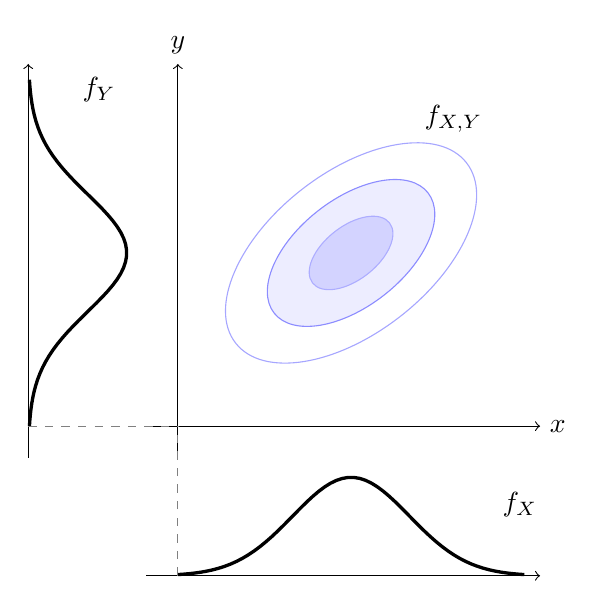
\begin{tikzpicture}[scale=1.0]
    % joint density: level sets of a correlated bivariate normal
    \begin{scope}[shift={(0,0)}]
      \draw[->] (-0.4,0) -- (4.6,0) node[right] {$x$};
      \draw[->] (0,-0.4) -- (0,4.6) node[above] {$y$};
      \begin{scope}[shift={(2.2,2.2)}, rotate=38]
        \draw[fill=blue!22, draw=blue!55] (0,0) ellipse (0.62 and 0.34);
        \draw[fill=blue!13, draw=blue!45, fill opacity=0.55] (0,0) ellipse (1.24 and 0.68);
        \draw[draw=blue!35] (0,0) ellipse (1.86 and 1.02);
      \end{scope}
      \node at (3.5,3.9) {$f_{X,Y}$};
    \end{scope}
    % marginal in x, drawn below the box
    \begin{scope}[shift={(0,-1.9)}]
      \draw[->] (-0.4,0) -- (4.6,0);
      \draw[very thick, black]
        plot[domain=0:4.4, samples=60] (\x, {1.25*exp(-(\x-2.2)*(\x-2.2)/1.1)});
      \node[right] at (4.0,0.9) {$f_{X}$};
    \end{scope}
    % marginal in y, drawn left of the box
    \begin{scope}[shift={(-1.9,0)}]
      \draw[->] (0,-0.4) -- (0,4.6);
      \draw[very thick, black]
        plot[domain=0:4.4, samples=60] ({1.25*exp(-(\x-2.2)*(\x-2.2)/1.1)}, \x);
      \node[above] at (0.9,4.0) {$f_{Y}$};
    \end{scope}
    \draw[dashed, gray] (0,-1.9) -- (0,0);
    \draw[dashed, gray] (-1.9,0) -- (0,0);
  \end{tikzpicture}
  \caption{A joint densité on $\reals^{2}$, shown by its level sets, with the two
  lois marginales obtained by integrating out the other coordinate. The lois
  marginales are projections and lose the tilt of the level sets: they cannot tell
  this loi from the independent one with the same two lois marginales.}
\end{figure}

\begin{example}[Reading marginals off a joint densité, and testing indépendance]
  Let $(X,Y)$ have densité
  $f_{X,Y}(x,y) = (x+y)\indic_{[0,1]^{2}}(x,y)$.
  It is non-negative, and it is a densité because
  \[
    \int_{\reals^{2}} (x+y)\indic_{[0,1]^{2}}(x,y)\,dx\,dy
    = \int_{0}^{1}\!\!\int_{0}^{1} (x+y)\,dx\,dy
    = 2\int_{0}^{1} x\,dx = 1 ,
  \]
  where the middle step uses the symmetry of the integrand in $x$ and $y$.
  Integrating out one coordinate,
  \[
    f_{X}(x) = \int_{0}^{1} (x+y)\,dy \cdot \indic_{[0,1]}(x)
             = \Big(x+\tfrac12\Big)\indic_{[0,1]}(x),
    \qquad
    f_{Y}(y) = \Big(y+\tfrac12\Big)\indic_{[0,1]}(y).
  \]
  Since $f_{X}(x)f_{Y}(y) = (x+\tfrac12)(y+\tfrac12) \neq x+y$ on a set of
  positive mesure, $X$ and $Y$ are \emph{not} independent. Note also that
  $\prob(X=Y)=0$, because $(X,Y)$ has a densité and the diagonal is négligeable
  for the mesure de Lebesgue in $\reals^{2}$; and by the symmetry of $f_{X,Y}$
  together with $\prob(X=Y)=0$, $\prob(X \leq Y) = \prob(X \geq Y) = \tfrac12$.
\end{example}

\subsection{Espérance}

Soit $X$ une variable aléatoire réelle.

\begin{definition}[Espérance]
  L'\textbf{espérance} de la variable aléatoire $X$ est le nombre éventuellement
  infini donné par :
  \[
    \expec(X) = \int X \,d\prob = \int_{\Omega} X(\omega)\,d\prob(\omega),
  \]
  dès que cette intégrale est bien définie.
\end{definition}

L'espérance est donc la moyenne des valeurs prises par $X$ lorsque $\omega$
parcourt $\Omega$. Cela généralise la notion d'espérance introduite dans le cas
discret, in chapter 1. The hypotheses are chapter 3's and must not be blurred:
\begin{itemize}
  \item l'espérance est toujours définie si $X \geq 0$ (elle peut être infinie,
    $+\infty$);
  \item en général, elle est bien définie si et seulement si
    $\expec(X^{+}) < \infty$ ou $\expec(X^{-}) < \infty$, and it is then
    $\expec(X^{+}) - \expec(X^{-})$;
  \item on dit que la variable aléatoire $X$ est intégrable si
    $\expec(|X|) < \infty$, which is the same as both parts being finite.
\end{itemize}
A variable can therefore have an espérance without being integrable (the loi de
Pareto with $a \leq 1$ has espérance $+\infty$), and it can fail to have one at all
(the loi de Cauchy). D'après le théorème de transfert, on a
\[
  \expec(X) = \int x \, d\prob_{X}(x) ,
\]
and l'espérance est donc le barycentre de la loi $\prob_{X}$; it depends on
nothing else about $X$.

\begin{example}[Espérance d'une variable de Bernoulli]
  Une variable aléatoire $X \sim \mathcal{B}(p)$, de paramètre $p \in [0,1]$, a
  pour espérance $\expec(X) = \int x\,d\prob_{X}(x) = \prob(X=1) = p$.
\end{example}

\begin{example}[Espérance of an indicator is a probability]
  Pour tout événement $A$, on a :
  \[
    \expec(\indic_{A}) = \int \indic_{A}\,d\prob = \prob(A).
  \]
  On a ici utilisé la définition de l'espérance, avec une intégrale par rapport à
  la mesure de probabilité $\prob$ --- an integral over $\Omega$. On obtient le
  même résultat en intégrant par rapport à la loi de la variable aléatoire
  $X=\indic_{A}$, qui est une loi de Bernoulli de paramètre $\prob(A)$ --- the
  transfer identity in its smallest case. This identity is used constantly: it is
  how a probability is turned into an integral so that Fubini or a changement de
  variable can act on it.
\end{example}

L'espérance hérite des propriétés de l'intégrale de Lebesgue.

\begin{theorem}
  Soit $X$, $Y$ deux variables aléatoires réelles. Alors :
  \begin{enumerate}
    \item $X = 0$ p.s.\ implique $\expec(X)=0$ ;
    \item $X = Y$ p.s.\ implique $\expec(X)=\expec(Y)$ dès que $X$ ou $Y$ a une
      espérance ;
    \item $X \geq 0$ p.s.\ implique $\expec(X) \geq 0$ ; si de plus
      $\expec(X)=0$ alors $X = 0$ p.s. ;
    \item $X \leq Y$ p.s.\ implique $\expec(X) \leq \expec(Y)$ dès que $X$ ou
      $Y$ a une espérance ; si de plus $\expec(X)=\expec(Y)$ alors
      $X = Y$ p.s.
  \end{enumerate}
\end{theorem}

The two converse halves of items 3 and 4 are used more often than they look.
``Non-negative with zero espérance forces the variable to vanish presque
sûrement'' is what turns an inequality between espérances into an almost-sure
statement, and it is the engine of the equality case in every one of the
inequalities that close this chapter.

\begin{theorem}[Linéarité]
  Soit $X$, $Y$ deux variables aléatoires réelles. Alors,
  \[
    \forall \alpha \in \reals, \qquad \expec(\alpha X) = \alpha\,\expec(X),
  \]
  et
  \[
    \expec(X+Y) = \expec(X) + \expec(Y),
  \]
  cette dernière égalité étant satisfaite dès que les variables aléatoires $X$,
  $Y$ sont positives ou que l'une d'elles est intégrable.
\end{theorem}

The side condition on additivity is not a technicality to be dropped. Without it
the right-hand side can be $(+\infty) + (-\infty)$, and the identity is
meaningless; positivity of both variables, or integrability of one of them, is
exactly what rules that out.

\begin{prop}[Espérance d'une série]
  Pour toute suite $(X_{n})_{n \geq 1}$ de variables aléatoires réelles,
  \[
    \expec\Big(\sum_{n \geq 1} X_{n}\Big) = \sum_{n \geq 1} \expec(X_{n})
  \]
  dès que les variables aléatoires $X_{n}$ sont positives pour tout $n \geq 1$,
  ou que $\sum_{n \geq 1} \expec(|X_{n}|) < \infty$.
\end{prop}

\begin{remark}
  These are the two standard hypotheses under which chapter 3 allows a sum and an
  integral to be exchanged: convergence monotone in the non-negative case,
  convergence dominée in the absolutely summable case. Either one alone
  suffices; neither can be dropped.
\end{remark}

\begin{example}[A series of espérances that diverges]
  Soit $(X_{n})_{n \geq 1}$ une suite de variables aléatoires telle que
  $X_{n} \sim \mathcal{B}(\tfrac1n)$. The variables are non-negative, so the
  exchange is legitimate without any integrability assumption, and
  \[
    \expec\Big(\sum_{n \geq 1} X_{n}\Big)
      = \sum_{n \geq 1} \frac{1}{n} = +\infty .
  \]
  No indépendance is needed, and the conclusion holds whatever the dependence
  between the $X_{n}$.
\end{example}

L'espérance hérite également de la propriété de transfert, from chapter 3. On
considère une variable aléatoire $X$ à valeurs dans un espace quelconque $E$,
muni d'une tribu $\mathcal{E}$.

\begin{theorem}[Transfert]
  Soit $X$ une variable aléatoire à valeurs dans $E$ et $\phi : E \to \reals$ une
  fonction mesurable. Alors,
  \[
    \expec(\phi(X)) = \int \phi(x)\,d\prob_{X}(x)
  \]
  dès que cette intégrale est bien définie.
\end{theorem}

This is the theorem that makes the loi sufficient. The left-hand side is an
integral over the abstract space $\Omega$; the right-hand side is an integral over
the value space against the loi. Since the loi is all one ever knows, every
computation below is a use of transfer, usually without saying so.

\begin{corollary}[Espérance du produit]
  Pour toutes variables aléatoires réelles $X$, $Y$ indépendantes d'espérances
  finies,
  \[
    \expec(XY) = \expec(X)\,\expec(Y).
  \]
\end{corollary}

\begin{remark}
  Apply transfer to the pair $(X,Y)$, whose loi is $\prob_{X} \otimes \prob_{Y}$
  by indépendance, and then Fubini. Run the argument first on $|xy|$, which is
  non-negative so Tonelli applies with no hypothesis, to get
  $\expec(|XY|) = \expec(|X|)\expec(|Y|) < \infty$; that finiteness is what
  licenses Fubini on $xy$ itself in the second pass. Skipping the first pass is
  the classic error --- Fubini needs integrability, and here integrability of the
  product is a conclusion, not an assumption. The converse of the corollary is
  false: $\expec(XY) = \expec(X)\expec(Y)$ does not imply indépendance.
\end{remark}

\paragraph{Cas des lois à densité.}
Soit $X$ une variable aléatoire réelle de densité $f_{X}$ par rapport à la mesure
de Lebesgue. On a :
\[
  \expec(X) = \int x f_{X}(x)\,dx
\]
dès que cette intégrale est bien définie. This is chapter 3's integration against
a mesure with a densité.

\begin{example}[Espérance d'une variable exponentielle]
  Soit $X \sim \mathcal{E}(\lambda)$ une variable aléatoire de loi exponentielle
  de paramètre $\lambda > 0$. Son espérance est :
  \[
    \expec(X) = \int_{0}^{+\infty} x \lambda e^{-\lambda x}\,dx = \frac{1}{\lambda}.
  \]
\end{example}

\begin{example}[A Pareto variable may have infinite espérance]
  Soit $X$ une variable aléatoire suivant une loi de Pareto de paramètre $a > 0$.
  Son espérance vaut :
  \[
    \expec(X) = \int_{1}^{+\infty} x \cdot \frac{a}{x^{a+1}}\,dx
    =
    \begin{cases}
      \dfrac{a}{a-1} & \text{if } a > 1,\\[6pt]
      +\infty & \text{otherwise.}
    \end{cases}
  \]
  The espérance exists in every case, because the variable is non-negative; it
  is finite only for $a>1$.
\end{example}

\begin{example}[A Cauchy variable has no espérance at all]
  Soit $X$ une variable aléatoire suivant une loi de Cauchy, de densité
  $f_{X}(x) = \frac{1}{\pi}\frac{1}{x^{2}+1}$. Comme
  $\expec(X^{+}) = \expec(X^{-}) = +\infty$, son espérance n'est pas définie: the
  difference would be $(+\infty)-(+\infty)$. This is the distinction between
  ``infinite espérance'' and ``no espérance'', and it matters: the law of large
  numbers has nothing to say here.
\end{example}

\begin{theorem}[Transfert pour les lois à densité]
  Soit $X$ une variable aléatoire de densité $f_{X}$ par rapport à la mesure de
  Lebesgue et $\phi : \reals \to \reals$ une fonction mesurable. Alors,
  \[
    \expec(\phi(X)) = \int \phi(x) f_{X}(x)\,dx
  \]
  dès que cette intégrale est bien définie.
\end{theorem}

This is the working form of transfer and the starting point of the fonction test
method below. Note what it does \emph{not} require: nothing about $\phi$ beyond
measurability --- no continuity, no monotonicity, no invertibility. It is the
absence of those requirements that makes the fonction test method universal.

\subsection{Variance, covariance}

Soit $X$ une variable aléatoire réelle d'espérance finie.

\begin{definition}[Variance]
  La \textbf{variance} de la variable aléatoire $X$ est la valeur, éventuellement
  infinie :
  \[
    \Var(X) = \expec\big((X-\expec(X))^{2}\big).
  \]
\end{definition}

Expanding the square, par linéarité, on a l'expression équivalente :
\[
  \Var(X) = \expec(X^{2}) - \expec(X)^{2},
\]
which is the one used in computations; the definition is the one used in proofs.

\begin{prop}
  On a $\Var(X) \geq 0$ avec $\Var(X) = 0$ si et seulement si $X = \expec(X)$ p.s.
\end{prop}

\begin{remark}
  C'est une conséquence directe of the theorem on the espérance above:
  $(X-\expec(X))^{2}$ is non-negative, so its espérance is non-negative, and a
  non-negative variable of zero espérance vanishes presque sûrement.
\end{remark}

Par linéarité de l'espérance, on a :
\[
  \forall \alpha \in \reals, \qquad \Var(\alpha X) = \alpha^{2}\,\Var(X),
\]
a scaling rule with the square on $\alpha$ --- the variance is not linear, and an
additive shift leaves it unchanged: $\Var(X+c) = \Var(X)$ for every constant
$c$.\\

On considère maintenant $X$ et $Y$ deux variables aléatoires réelles
d'espérances finies.

\begin{definition}[Covariance]
  La \textbf{covariance} entre les variables aléatoires $X$ et $Y$ est la
  valeur :
  \[
    \Cov(X,Y) = \expec\big((X-\expec(X))(Y-\expec(Y))\big).
  \]
\end{definition}

Par linéarité de l'espérance, on a :
\[
  \Cov(X,Y) = \expec(XY) - \expec(X)\,\expec(Y).
\]
On note que $\Cov(X,Y)=0$ dès que $X$ et $Y$ sont indépendantes, by the corollary
on the espérance du produit. \textbf{La réciproque est fausse}, and the standard
counter-example is worth carrying.

\begin{example}[Uncorrelated but dependent]
  Let $X$ be uniform on $[-1,1]$ and $Y = X^{2}$. Then $\expec(X)=0$ and
  $\expec(XY) = \expec(X^{3}) = 0$ by symmetry, so $\Cov(X,Y)=0$. But $Y$ is a
  function of $X$, so the pair is as dependent as it can be: the événements
  $\{Y \leq \tfrac14\}$ and $\{|X| \leq \tfrac12\}$ are one and the same, so
  $\prob(Y \leq \tfrac14,\ |X| \leq \tfrac12) = \tfrac12$ while the product of
  the two probabilities is
  $\prob(Y \leq \tfrac14)\,\prob(|X| \leq \tfrac12) = \tfrac14$: the product rule
  of the definition of indépendance fails outright. Zero covariance only says the
  best linear predictor of $Y$ from $X$ is constant.
\end{example}

La covariance vérifie les propriétés suivantes :
\begin{itemize}
  \item $\Cov(X,X) = \Var(X)$;
  \item $\Cov(X,Y) = \Cov(Y,X)$;
  \item $\Cov(\alpha X, Y) = \alpha \Cov(X,Y)$ pour tout $\alpha \in \reals$;
  \item $\Cov(X, Y+Z) = \Cov(X,Y) + \Cov(X,Z)$ pour toutes variables $X,Y,Z$ de
    variances finies.
\end{itemize}
La covariance est donc une forme bilinéaire symétrique on the space of variables
with finite variance, and the variance is its associated quadratic form.
Expanding that quadratic form gives the identity the whole of chapter 8 rests on;
en particulier, on a
\[
  \boxed{\;\Var(X+Y) = \Var(X) + 2\Cov(X,Y) + \Var(Y)\;}
\]
pour toutes variables aléatoires $X$, $Y$ de variances finies. Si les variables
aléatoires $X$ et $Y$ sont indépendantes, it collapses to
\[
  \Var(X+Y) = \Var(X) + \Var(Y)
\]
On définit le coefficient de corrélation comme dans le cas discret:
$\rho(X,Y) = \Cov(X,Y)/\sqrt{\Var(X)\Var(Y)}$ when both variances are finite and
non-zero; it lies in $[-1,1]$ by the inégalité de Cauchy-Schwartz.

\begin{example}[A covariance computed by splitting on a discrete factor]
  Let $X$ be uniform on $[-1,1]$ and $Y$ uniform on $\{1,2\}$, independent, and
  set $Z = X^{Y}$. Conditioning on the two values of $Y$, each of probability
  $\tfrac12$,
  \[
    \expec(Z) = \tfrac12\big(\expec(X) + \expec(X^{2})\big) = \tfrac12\expec(X^{2}),
    \qquad
    \expec(X^{2}) = \int_{-1}^{1} x^{2}\,\tfrac12\,dx = \tfrac13 ,
  \]
  so $\expec(Z) = \tfrac16$. The same split gives
  \[
    \expec(XZ) = \expec(X^{Y+1})
      = \tfrac12\big(\expec(X^{2}) + \expec(X^{3})\big)
      = \tfrac12 \expec(X^{2}) = \tfrac16 ,
  \]
  since $\expec(X^{3})=0$ by symmetry. As $\expec(X)=0$,
  $\Cov(X,Z) = \expec(XZ) - \expec(X)\expec(Z) = \tfrac16$. Two things are doing
  the work: indépendance of $X$ and $Y$, which lets each espérance conditionnelle
  be computed as an unconditional one; and the symmetry of the loi uniforme on
  $[-1,1]$, which kills every odd moment.
\end{example}

\subsection{Vecteurs aléatoires}

Les résultats vus jusqu'à présent se généralisent au cas des vecteurs aléatoires,
from $\reals$ to $\reals^{n}$, and the generalisation is where the linear algebra
enters.

\begin{definition}[Vecteur aléatoire]
  Un \textbf{vecteur aléatoire} $X$ est une variable aléatoire à valeurs dans
  l'ensemble $\reals^{n}$ muni de la tribu de Borel, pour un certain entier
  $n \geq 1$.
\end{definition}

On note $X_{1},\dots,X_{n}$ les composantes de $X$. Ce sont des variables
aléatoires réelles. La loi de $X$ est la loi jointe des variables aléatoires
$X_{1},\dots,X_{n}$ ; les lois de $X_{1},\dots,X_{n}$ sont les lois marginales du
vecteur aléatoire. Pour tous vecteurs $x,y \in \reals^{n}$, on note $x \leq y$
l'inégalité composante par composante.

\begin{definition}[Fonction de répartition d'un vecteur aléatoire]
  La \textbf{fonction de répartition} d'un vecteur aléatoire $X$ à valeurs dans
  $\reals^{n}$ est la fonction $F_{X}$ définie par :
  \[
    \forall x \in \reals^{n}, \qquad F_{X}(x) = \prob(X \leq x).
  \]
\end{definition}

Comme dans le cas des variables aléatoires réelles, $F_{X}$ est une fonction
croissante, continue à droite, qui tend vers $0$ lorsque toutes les composantes de
$x$ tendent vers $-\infty$ et vers $1$ lorsque toutes les composantes tendent vers
$+\infty$.

\begin{definition}[Vecteur à densité]
  Un vecteur aléatoire $X$ à valeurs dans $\reals^{n}$ a pour \textbf{densité} la
  fonction $f_{X}$ par rapport à la mesure de Lebesgue si :
  \[
    \forall A \in \mathcal{B}(\reals^{n}), \qquad
    \prob_{X}(A) = \int_{A} f_{X}(x)\,dx .
  \]
\end{definition}

La fonction de densité est mesurable, positive, et telle que
$\int_{\reals^{n}} f_{X}(x)\,dx = 1$. Par le théorème de Fubini, les lois
marginales ont également une densité, obtenues en intégrant la densité de $X$ sur
les autres variables.

\begin{remark}[The mesure de référence]
  Lorsque la mesure de référence n'est pas précisée, il s'agit par convention de
  la mesure de Lebesgue. Les résultats s'étendent à n'importe quel produit de
  mesures \emph{$\sigma$-finies} --- that hypothesis is what Fubini needs and it
  is not automatic; it is satisfied by the mesure de Lebesgue on $\reals^{n}$ and
  by the mesure de comptage on a countable set.
\end{remark}

\begin{prop}
  Si le vecteur $X$ a une densité, alors
  \[
    \forall i \neq j, \qquad \prob(X_{i}=X_{j}) = 0.
  \]
\end{prop}

\begin{remark}
  Les ensembles $\{x \in \reals^{n} : x_{i}=x_{j}\}$ pour tous $i \neq j$ ---
  hyperplanes --- étant négligeables pour la mesure de Lebesgue, c'est une
  conséquence du fait que la loi de $X$ est absolument continue par rapport à la
  mesure de Lebesgue: it gives them mass zero. This is the quickest way to see
  that a vector cannot have a densité when two of its components coincide.
\end{remark}

\begin{example}[Two independent uniforms never collide]
  Soit $X$ un vecteur de loi uniforme sur $[0,1]^{2}$. Alors
  $\prob(X_{1}=X_{2})=0$ : the diagonal is a segment in the square, of area zero.
  Contrast the vector $(U,U)$ with $U$ uniform on $[0,1]$, which lives entirely on
  that diagonal and therefore has no densité at all, even though each of its two
  lois marginales has one.
\end{example}

\paragraph{Espérance.}

La notion d'espérance se généralise aux vecteurs aléatoires réels, componentwise.

\begin{definition}[Espérance d'un vecteur aléatoire]
  L'\textbf{espérance} du vecteur aléatoire $X$ est le vecteur des espérances :
  \[
    \expec(X) = \begin{pmatrix} \expec(X_{1}) \\ \vdots \\ \expec(X_{n}) \end{pmatrix}.
  \]
  Elle est définie si et seulement si toutes les composantes du vecteur $X$ ont
  une espérance.
\end{definition}

\begin{prop}[Linéarité de l'espérance]
  Soit $X$, $Y$ des vecteurs aléatoires à valeurs dans $\reals^{n}$ d'espérances
  finies. Alors, pour toute matrice $A$,
  \[
    \expec(AX) = A\,\expec(X)
    \qquad\text{and}\qquad
    \expec(X+Y) = \expec(X)+\expec(Y).
  \]
\end{prop}

\begin{remark}
  Each coordinate of $AX$ is a finite linear combination of the $X_{i}$: c'est une
  conséquence directe de la linéarité de l'espérance pour les variables
  aléatoires réelles, applied $n$ times. The finiteness of the espérances is what
  makes those combinations legitimate --- the scalar theorem's side condition,
  inherited.
\end{remark}

\paragraph{Matrice de covariance.}

Les notions de variance et de covariance se généralisent également aux vecteurs
aléatoires réels, and they do so together: the $n^{2}$ pairwise covariances of the
components are collected into a single matrix.

\begin{definition}[Matrice de covariance]
  Soit $X$ un vecteur aléatoire à valeurs dans $\reals^{n}$ d'espérance finie. La
  \textbf{matrice de covariance} (\textit{covariance matrix}) de $X$ est la
  matrice des covariances de ses composantes :
  \[
    \Cov(X) = \big(\Cov(X_{i},X_{j})\big)_{1 \leq i,j \leq n}.
  \]
\end{definition}

On notera les deux propriétés suivantes, used constantly. La diagonale de la
matrice de covariance est le vecteur des variances, since
$\Cov(X_{i},X_{i}) = \Var(X_{i})$. Si les variables aléatoires
$X_{1},\dots,X_{n}$ sont indépendantes, la matrice de covariance est diagonale ---
the converse being false, by the example above of décorrélées but dependent
variables, except for the vecteurs gaussiens of chapter 7. En généralisant la
notion d'espérance à une matrice, entrywise, on obtient l'expression matricielle :
\[
  \Cov(X) = \expec\big((X-\expec(X))(X-\expec(X))^{T}\big).
\]

\begin{prop}
  La matrice de covariance est symétrique positive.
\end{prop}

\begin{remark}
  La matrice de covariance est symétrique car
  $\Cov(X_{i},X_{j}) = \Cov(X_{j},X_{i})$. Par ailleurs, for the quadratic form,
  on a pour tout $a \in \reals^{n}$ :
  \[
    a^{T}\Cov(X)a
      = a^{T}\expec\big((X-\expec(X))(X-\expec(X))^{T}\big)a
      = \expec\big((a^{T}(X-\expec(X)))^{2}\big) \geq 0 ,
  \]
  the middle step being the linéarité de l'espérance applied to the constant
  matrix $a^{T}$ on each side. ``Positive'' here means positive
  \emph{semi}-definite: the form vanishes on $a$ exactly when
  $a^{T}X$ is presque sûrement constant, which happens whenever the components
  satisfy an affine relation. Chapter 7 is where the distinction between
  definite and semi-definite becomes the difference between a vecteur gaussien
  with a densité and one without.
\end{remark}

\begin{definition}[Matrice de covariance entre vecteurs]
  Soit $X$, $Y$ deux vecteurs aléatoires à valeurs dans $\reals^{n}$ d'espérances
  finies. La \textbf{matrice de covariance entre $X$ et $Y$} est la matrice des
  covariances de leurs composantes :
  \[
    \Cov(X,Y) = \big(\Cov(X_{i},Y_{j})\big)_{1 \leq i,j \leq n}.
  \]
\end{definition}

On note que $\Cov(X,Y)=0$ dès que les vecteurs $X$ et $Y$ sont indépendants. Par
ailleurs,
\[
  \Cov(X) = \Cov(X,X), \qquad \Cov(Y,X) = \Cov(X,Y)^{T},
\]
et on a l'expression matricielle :
\[
  \Cov(X,Y) = \expec\big((X-\expec(X))(Y-\expec(Y))^{T}\big).
\]
Note that $\Cov(X,Y)$ is not symétrique in general; only $\Cov(X)$ is.

\begin{prop}[Bilinéarité de la covariance]
  Soit $X$, $Y$ des vecteurs aléatoires à valeurs respectives dans $\reals^{n}$,
  $\reals^{m}$, d'espérances finies. Pour toute matrice
  $A \in \reals^{m \times n}$,
  \[
    \Cov(AX,Y) = A\,\Cov(X,Y),
    \qquad
    \Cov(Y,AX) = \Cov(Y,X)A^{T}.
  \]
  Par ailleurs, pour tous vecteurs aléatoires $X,Y,Z$ à valeurs dans $\reals^{n}$,
  \[
    \Cov(X+Y,Z) = \Cov(X,Z)+\Cov(Y,Z),
    \qquad
    \Cov(Z,X+Y) = \Cov(Z,X)+\Cov(Z,Y).
  \]
\end{prop}

\begin{remark}
  All four identities are une conséquence directe de la linéarité de l'espérance
  for vectors, applied inside the matrix expression above. The transpose in the
  second identity is forced by the shape of the matrices and is the most common
  slip.
\end{remark}

\begin{prop}[Covariance d'une somme]
  Pour tous vecteurs aléatoires $X$, $Y$ sur $\reals^{n}$,
  \[
    \Cov(X+Y) = \Cov(X) + \Cov(Y) + \Cov(X,Y) + \Cov(Y,X).
  \]
  En particulier, on a pour tous vecteurs aléatoires indépendants $X$, $Y$ sur
  $\reals^{n}$,
  \[
    \Cov(X+Y) = \Cov(X) + \Cov(Y).
  \]
\end{prop}

This is the vector form of the scalar variance-of-a-sum identity above, and it
is worth writing both
out side by side, because chapter 8's normalisation of a sum is nothing but these
two lines:
\[
  \Var(X+Y) = \Var(X) + \Var(Y) + 2\Cov(X,Y),
\]
\[
  \Cov(X+Y) = \Cov(X) + \Cov(Y) + \Cov(X,Y) + \Cov(X,Y)^{T} .
\]
In the scalar case the two cross terms coincide and give the factor $2$; in the
vector case they are transposes of each other and cannot be merged. Applied to
$n$ independent variables with the same variance $\sigma^{2}$, the first line
gives $\Var(X_{1}+\dots+X_{n}) = n\sigma^{2}$, hence an écart type growing like
$\sqrt{n}$ --- which is exactly the normalisation the théorème central limite
divides by.

\subsection{Variables aléatoires indépendantes}

La notion d'indépendance entre deux variables aléatoires vue précédemment se
généralise au cas de $n$ variables aléatoires, and the characterisations for two
variables generalise with it. Les preuves des résultats suivants sont identiques
à celles vues pour deux variables, with rectangles of two factors replaced by
rectangles of $n$.

\begin{definition}[Indépendance de $n$ variables aléatoires]
  Les variables aléatoires réelles $X_{1},\dots,X_{n}$ sont dites
  \textbf{indépendantes} si pour tous $A_{1},\dots,A_{n} \in \mathcal{B}(\reals)$,
  les événements $\{X_{1} \in A_{1}\},\dots,\{X_{n} \in A_{n}\}$ sont
  indépendants.
\end{definition}

The événements being independent means every sub-family has a product
probability, not merely the whole family --- pairwise indépendance is strictly
weaker and is not what is meant here.

\begin{theorem}[Caractérisation de l'indépendance]
  Les propositions suivantes sont équivalentes :
  \begin{itemize}
    \item les variables aléatoires réelles $X_{1},\dots,X_{n}$ sont
      indépendantes ;
    \item leur loi jointe est le produit des lois marginales :
      \[
        \prob_{X} = \prob_{X_{1}} \otimes \dots \otimes \prob_{X_{n}} ;
      \]
    \item la fonction de répartition du vecteur $X$ est le produit des fonctions
      de répartition des lois marginales :
      \[
        \forall x \in \reals^{n}, \qquad
        F_{X}(x) = F_{X_{1}}(x_{1}) \dots F_{X_{n}}(x_{n}).
      \]
  \end{itemize}
\end{theorem}

The third characterisation is the practical one: it reduces an indépendance check
to an algebraic factorisation of a function of $n$ real variables.

\begin{theorem}[Indépendance et densité]
  Soit $X$ un vecteur aléatoire à valeurs dans $\reals^{n}$ de densité $f_{X}$
  par rapport à la mesure de Lebesgue. Les propositions suivantes sont
  équivalentes :
  \begin{itemize}
    \item les variables aléatoires réelles $X_{1},\dots,X_{n}$ sont
      indépendantes ;
    \item la densité de $X$ est le produit des densités des lois marginales :
      \[
        \forall x \in \reals^{n}, \qquad
        f_{X}(x) = f_{X_{1}}(x_{1}) \dots f_{X_{n}}(x_{n}) \quad \text{p.p.}
      \]
  \end{itemize}
\end{theorem}

The hypothesis that $X$ \emph{has} a densité is part of the statement and cannot
be dropped: without it there is nothing to factorise. Note too that the
factorisation need only hold presque partout, and that it suffices to exhibit
$f_{X}$ as a product of a function of $x_{1}$ alone, \ldots, a function of
$x_{n}$ alone --- the factors are then automatically the marginal densités up to
constants that multiply to one.

\begin{example}[The loi uniforme on a cube has independent coordinates]
  Soit $X$ le vecteur aléatoire de loi uniforme sur $[0,1]^{n}$. Its densité
  factorises,
  \[
    \forall x \in \reals^{n}, \qquad
    f_{X}(x) = \indic_{[0,1]^{n}}(x) = \indic_{[0,1]}(x_{1}) \dots \indic_{[0,1]}(x_{n}),
  \]
  so ses composantes $X_{1},\dots,X_{n}$ sont indépendantes, chacune de loi
  uniforme sur $[0,1]$. The factorisation of an indicator of a product set is the
  most common instance of the criterion, and the reason an indicator of a
  \emph{non}-product set --- a triangle, a disc, the region $\{x < y\}$ ---
  signals dependence at a glance.
\end{example}

\begin{prop}[Existence d'une densité pour un vecteur]
  Soit $X$ un vecteur aléatoire dont les composantes sont indépendantes. Si chaque
  loi marginale a une densité, la loi jointe a une densité, donnée par :
  \[
    \forall x \in \reals^{n}, \qquad
    f_{X}(x) = f_{X_{1}}(x_{1}) \dots f_{X_{n}}(x_{n}) \quad \text{p.p.}
  \]
\end{prop}

\begin{example}[Indépendance is what makes the joint densité exist]
  Soit $X$, $Y$ des variables aléatoires indépendantes de même loi uniforme sur
  $[0,1]$. Alors le vecteur aléatoire $(X,Y)$ a une densité par rapport à la
  mesure de Lebesgue sur $\reals^{2}$, égale à $\indic_{[0,1]^{2}}$. Ce n'est pas
  le cas du vecteur $(X,X)$, by the hyperplane argument above, although its two
  components have exactly the same lois marginales. The lois marginales never
  determine the loi jointe; indépendance is one extra piece of information that
  does.
\end{example}

\subsection{Calcul de densité}

This section is one proposition and a procedure, and it is the most-used
calculation on this syllabus. Soit $X$ une variable aléatoire réelle ayant une
densité $f_{X}$. Par le théorème de transfert, on a pour toute fonction mesurable
positive $\phi$ :
\[
  \expec(\phi(X)) = \int \phi(x) f_{X}(x)\,dx .
\]
Il s'avère que cette propriété est une condition nécessaire et suffisante --- not
merely necessary but sufficient: it \emph{characterises} the densité. La fonction
$\phi$, que l'on n'explicite pas, s'appelle la \textbf{fonction test} (\textit{test function}), as in the chapter
opening. Le résultat s'étend aux vecteurs aléatoires, verbatim.

\begin{prop}[Fonction test]
  Une variable aléatoire réelle ou un vecteur aléatoire réel $X$ a pour densité
  la fonction $f_{X}$ si et seulement si pour toute fonction mesurable positive
  $\phi$ :
  \[
    \expec(\phi(X)) = \int \phi(x) f_{X}(x)\,dx .
  \]
\end{prop}

\begin{proof}
  La condition nécessaire vient du théorème de transfert pour les lois à densité.
  Pour la condition suffisante, il suffit d'appliquer l'égalité à la fonction
  indicatrice $\phi = \indic_{A}$, pour tout borélien $A$, which is non-negative
  and mesurable and therefore an admissible fonction test. On obtient :
  \[
    \prob(X \in A) = \expec(\indic_{A}(X)) = \int_{A} f_{X}(x)\,dx ,
  \]
  for every $A$, ce qui montre que $X$ a pour densité la fonction $f_{X}$.
\end{proof}

The proof is three lines, and it is worth seeing why it is so short: the class of
fonctions test is large enough to contain the indicators, and the indicators are
already the definition of a densité. Everything else is bookkeeping.

\begin{remark}[The method, as a procedure]
  To find the densité of $Y = g(X)$, where the loi of $X$ is known:
  \begin{enumerate}
    \item Take an arbitrary non-negative mesurable fonction test $\phi$ and
      write $\expec(\phi(Y)) = \expec(\phi(g(X)))$.
    \item Expand the right-hand side by transfer, as an integral of
      $\phi(g(x))$ against the known densité of $X$.
    \item Change variables --- $y = g(x)$, or a diffeomorphism in the vector case ---
      so that the integral becomes $\int \phi(y)\,h(y)\,dy$ with $\phi$
      evaluated at the integration variable and nothing else depending on
      $\phi$.
    \item Read off $f_{Y} = h$. The indicator of the image domain is part of $h$
      and must be carried through the changement de variable; forgetting it is
      the commonest error.
  \end{enumerate}
  If step 3 cannot be completed --- if a term survives in which $\phi$ is
  evaluated at a fixed point --- the loi has an atom there and no densité
  exists. That failure is informative, not a dead end.
\end{remark}

Ce n'est pas la seule méthode ; on peut par exemple calculer la fonction de
répartition puis la dériver lorsque c'est possible, and for a monotone $g$ that is
often quicker. Mais la méthode de la fonction test présente l'avantage d'être
applicable à tous les cas, y compris vectoriels --- where there is no fonction de
répartition worth differentiating --- and it needs no monotonicity or
invertibility of $g$.

\begin{example}[The square of a uniform variable]
  Soit $X = U^{2}$ où $U$ suit une loi uniforme sur $[0,1]$. Pour toute fonction
  mesurable positive $\phi$,
  \[
    \expec(\phi(X)) = \expec(\phi(U^{2}))
      = \int \phi(u^{2}) \indic_{]0,1[}(u)\,du
      = \int \phi(x) \frac{\indic_{]0,1[}(x)}{2\sqrt{x}}\,dx ,
  \]
  substituting $x = u^{2}$, so $u = \sqrt{x}$ and $du = dx/(2\sqrt{x})$. Hence
  \[
    \forall x \in \reals, \qquad f_{X}(x) = \frac{\indic_{]0,1[}(x)}{2\sqrt{x}} .
  \]
  The densité is unbounded at $0$, which is perfectly legal --- a densité need
  only be mesurable, non-negative and integrate to $1$.
\end{example}

\begin{example}[A vector densité by a changement de variable]
  Soit $U$, $V$ deux variables aléatoires i.i.d.\ de loi uniforme sur $[0,1]$, and
  set
  \[
    X = UV, \qquad Y = \frac{V}{U} .
  \]
  Take a fonction test $\phi$, non-negative and mesurable on $\reals^{2}$. Since
  $(U,V)$ has densité $\indic_{]0,1[^{2}}$,
  \[
    \expec(\phi(X,Y))
      = \expec\!\left(\phi\!\left(UV, \frac{V}{U}\right)\right)
      = \int \phi\!\left(uv, \frac{v}{u}\right)\indic_{]0,1[^{2}}(u,v)\,du\,dv .
  \]
  On procède au changement de variable $x = uv$, $y = v/u$, correspondant au
  difféomorphisme
  \[
    \psi : \left]0,1\right[^{2} \longrightarrow \Delta,
    \qquad
    (u,v) \longmapsto \left(uv, \frac{v}{u}\right),
    \qquad
    \Delta = \Big\{(x,y) \in \reals^{2} : 0 < x < \min\Big(y,\tfrac{1}{y}\Big)\Big\},
  \]
  de matrice jacobienne
  \[
    J_{\psi} =
    \begin{pmatrix}
      v & u \\[2pt] -\dfrac{v}{u^{2}} & \dfrac{1}{u}
    \end{pmatrix},
    \qquad
    |\det J_{\psi}| = \frac{v}{u} + \frac{uv}{u^{2}} = \frac{2v}{u} = 2y .
  \]
  Chapter 3's changement de variable theorem then gives
  \[
    \expec(\phi(X,Y)) = \int \phi(x,y)\,\frac{\indic_{\Delta}(x,y)}{2y}\,dx\,dy ,
  \]
  so
  \[
    \forall (x,y) \in \reals^{2}, \qquad
    f_{X,Y}(x,y) = \frac{\indic_{\Delta}(x,y)}{2y} .
  \]
  The densité does not factorise --- the domain $\Delta$ is not a product set ---
  so $X$ and $Y$ are not independent, which one can see before computing anything
  else.
\end{example}

\begin{example}[When the method fails, it says why]
  Soit $X = \min(U,\tfrac12)$ où $U$ suit une loi uniforme sur $[0,1]$. Il est
  clair que la variable aléatoire n'a pas de densité puisque sa loi a un atome en
  $\tfrac12$, of mass $\tfrac12$. Running the method anyway: si on tente
  d'appliquer la méthode de la fonction test, on obtient pour toute fonction
  mesurable positive $\phi$ :
  \[
    \expec(\phi(X)) = \int \phi\!\left(\min\!\left(u,\tfrac12\right)\right)\indic_{]0,1[}(u)\,du
      = \int \phi(u)\indic_{]0,1/2[}(u)\,du + \frac{\phi(\tfrac12)}{2} .
  \]
  The second term cannot be written as $\int \phi(x) h(x)\,dx$ for any function
  $h$, because it depends on $\phi$ only through its value at a single point.
  That surviving term \emph{is} the atom, and its coefficient is the atom's mass.
\end{example}

\begin{example}[The ratio of the two pieces of a broken stick]
  A stick of length $1$ is broken at a point $U$ uniform on $]0,1[$. Let $R$ be
  the ratio of the shorter piece to the longer one, that is
  \[
    R = \frac{\min(U,1-U)}{\max(U,1-U)} \in \left]0,1\right[ .
  \]
  The loi of $U$ is symétrique about $\tfrac12$, so for any non-negative
  mesurable $\phi$ the two halves contribute equally and
  \[
    \expec(\phi(R)) = 2\int_{0}^{1/2} \phi\!\left(\frac{u}{1-u}\right) du .
  \]
  Substitute $r = u/(1-u)$, so that $u = r/(1+r)$ and
  $du = dr/(1+r)^{2}$, and $u \in \left]0,\tfrac12\right[$ corresponds to
  $r \in \left]0,1\right[$:
  \[
    \expec(\phi(R)) = \int \phi(r)\,\frac{2\,\indic_{]0,1[}(r)}{(1+r)^{2}}\,dr ,
    \qquad\text{hence}\qquad
    f_{R}(r) = \frac{2}{(1+r)^{2}}\,\indic_{]0,1[}(r).
  \]
  The espérance follows by transfer, splitting the numerator as
  $2r = 2(1+r) - 2$:
  \[
    \expec(R) = \int_{0}^{1} \frac{2r}{(1+r)^{2}}\,dr
      = \int_{0}^{1} \frac{2}{1+r}\,dr - \int_{0}^{1} \frac{2}{(1+r)^{2}}\,dr
      = 2\ln 2 - 1 \approx 0.386 .
  \]
  The same answer can be had by computing $F_{R}$ directly and differentiating;
  the fonction test spares the case analysis.
\end{example}

\begin{example}[A densité under a linear change of coordinates]
  Let $(X,Y)$ have densité $f_{X,Y}(x,y) = (x+y)\indic_{[0,1]^{2}}(x,y)$, and
  look for the densité of the vector $(X, X+Y)$. For $\phi$ non-negative and
  mesurable on $\reals^{2}$,
  \[
    \expec(\phi(X,X+Y)) = \int \phi(x,x+y)(x+y)\indic_{[0,1]^{2}}(x,y)\,dx\,dy .
  \]
  Substitute $z = x+y$ at fixed $x$, a translation whose Jacobian determinant is
  $1$; the constraint $y \in [0,1]$ becomes $z \in [x,x+1]$, and the integrand's
  factor $(x+y)$ becomes $z$:
  \[
    \expec(\phi(X,X+Y)) = \int \phi(x,z)\, z\, \indic_{[0,1]}(x)\indic_{[x,x+1]}(z)\,dx\,dz ,
  \]
  so
  \[
    f_{X,X+Y}(x,z) = z\,\indic_{[0,1]}(x)\,\indic_{[x,x+1]}(z).
  \]
  As a check, $\int_{0}^{1}\!\int_{x}^{x+1} z\,dz\,dx = \int_{0}^{1}(x+\tfrac12)\,dx = 1$.
  The support is a tilted band, not a rectangle, so the two components are not
  independent --- a linear change of coordinates that mixes the variables almost
  always destroys indépendance, and the indicator is where one sees it.
\end{example}

\subsection{Inégalités}

On termine ce chapitre par quelques inégalités utiles, four of them. They are
short, their proofs are reusable, and between them they are the standard route to
a weak law of large numbers. Chapter 8 proves the loi forte des grands nombres by a
fourth-moment expansion instead, and reaches for Markov only in its
exponential-bound example --- but the habit of bounding a probability by a moment
is the one to take from here.

\begin{prop}[Inégalité de Markov (\textit{Markov's inequality})]
  Soit $X$ une variable aléatoire réelle \emph{positive}. Alors,
  \[
    \forall a > 0, \qquad \prob(X \geq a) \leq \frac{\expec(X)}{a}.
  \]
\end{prop}

\begin{proof}
  For every $a > 0$, the pointwise inequality
  \[
    \indic_{\{X \geq a\}} \leq \frac{X}{a}
  \]
  holds: on $\{X \geq a\}$ the left side is $1$ and the right side is at least
  $1$; off that événement the left side is $0$ and the right side is
  non-negative, which is where the hypothesis $X \geq 0$ is used. La preuve en
  découle en prenant l'espérance, which preserves the inequality by monotonicity:
  $\prob(X \geq a) \leq \expec(X)/a$.
\end{proof}

The positivity hypothesis is not decorative. Without it the pointwise inequality
fails off the événement, and the conclusion is false: a variable equal to $-M$
with probability $\tfrac12$ and to $a$ with probability $\tfrac12$ has
$\prob(X \geq a) = \tfrac12$ and an espérance that can be made arbitrarily
negative. In practice one applies Markov not to $X$ but to $|X|$, to $|X|^{p}$ or
to $e^{\theta X}$ --- each choice is non-negative by construction and each gives a
different, and generally sharper, tail bound.

\begin{figure}[htbp]
  \centering
  % left panel: the tail of a density
  \begin{minipage}[b]{0.46\textwidth}
    \centering
    \begin{tikzpicture}
      \begin{axis}[
        width=6.6cm, height=4.4cm,
        axis lines=left,
        xlabel={$x$}, ylabel={$f_{X}(x)$},
        xmin=0, xmax=4.4, ymin=0, ymax=1.08,
        xtick={1.6}, xticklabels={$a$}, ytick=\empty,
        ]
        \addplot[name path=ft, domain=1.6:4.4, samples=60, draw=none] {exp(-x)};
        \addplot[name path=at, domain=1.6:4.4, samples=2, draw=none] {0};
        \addplot[fill=red!25] fill between[of=ft and at];
        \addplot[very thick, black, domain=0:4.4, samples=110] {exp(-x)};
        \node at (axis cs:2.9,0.30) {\small $\prob(X \geq a)$};
      \end{axis}
    \end{tikzpicture}

    {\small (a) the tail événement}
  \end{minipage}
  \hfill
  % right panel: a 1_{x>=a} <= x
  \begin{minipage}[b]{0.50\textwidth}
    \centering
    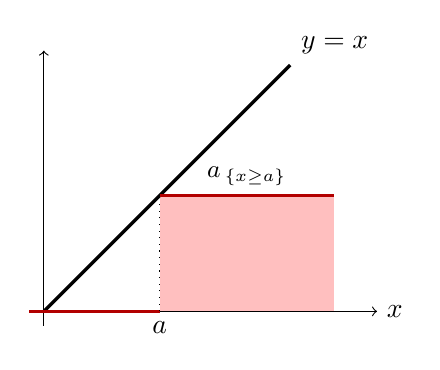
\begin{tikzpicture}[scale=0.92]
      \draw[->] (-0.2,0) -- (4.6,0) node[right] {$x$};
      \draw[->] (0,-0.2) -- (0,3.6);
      \fill[red!25] (1.6,0) rectangle (4.0,1.6);
      \draw[very thick, black] (0,0) -- (3.4,3.4) node[above right] {$y=x$};
      \draw[very thick, red!70!black] (-0.2,0) -- (1.6,0);
      \draw[very thick, red!70!black] (1.6,1.6) -- (4.0,1.6);
      \draw[dotted] (1.6,0) -- (1.6,1.6);
      \node[below] at (1.6,0) {$a$};
      \node[above] at (2.8,1.6) {\small $a\,\indic_{\{x \geq a\}}$};
    \end{tikzpicture}

    {\small (b) $a\,\indic_{\{X \geq a\}} \leq X$}
  \end{minipage}
  \caption{Inégalité de Markov. The rectangle of height $a$ over the tail sits
  under the line $y=x$, so taking espérances gives
  $a\,\prob(X \geq a) \leq \expec(X)$. The picture is the proof, and it is also
  where the hypothesis $X \geq 0$ enters: for negative $x$ the line dips below
  the axis and the domination fails.}
\end{figure}

\begin{prop}[Inégalité de Tchebychev (\textit{Tchebychev's inequality})]
  Soit $X$ une variable aléatoire réelle intégrable. Alors,
  \[
    \forall a > 0, \qquad \prob(|X - \expec(X)| \geq a) \leq \frac{\Var(X)}{a^{2}}.
  \]
\end{prop}

\begin{proof}
  Il suffit d'appliquer l'inégalité de Markov à la variable aléatoire
  $(X-\expec(X))^{2}$, which is non-negative as required, at the level
  $a^{2} > 0$ :
  \[
    \prob(|X-\expec(X)| \geq a)
      = \prob\big((X-\expec(X))^{2} \geq a^{2}\big)
      \leq \frac{\expec\big((X-\expec(X))^{2}\big)}{a^{2}}
      = \frac{\Var(X)}{a^{2}} .
  \]
  The first equality is the equivalence $|t| \geq a \iff t^{2} \geq a^{2}$ for
  $a>0$.
\end{proof}

Integrability of $X$ is what makes $\expec(X)$ exist, so that the statement can be
written at all; the bound is vacuously true when $\Var(X) = +\infty$ and carries
information only when the variance is finite. The shape $\Var(X)/a^{2}$ is the
reason Tchebychev, not Markov, gives the weak law of large numbers: applied to an
average of $n$ independent variables, the variance in the numerator carries a
factor $1/n$ and the bound goes to zero.

\begin{example}[A crude but universal bound on a Gaussian tail]
  Soit $X \sim \mathcal{N}(0,1)$ une variable aléatoire suivant une loi normale
  centrée réduite, so $\expec(X)=0$ and $\Var(X)=1$. Alors,
  \[
    \forall a > 0, \qquad \prob(|X| \geq a) \leq \frac{1}{a^{2}} .
  \]
  At $a=3$ this gives $\tfrac19 \approx 0.111$ against the true value
  $\approx 0.0027$: Tchebychev is far from sharp for a loi gaussienne, because it
  uses only two moments. Its value is that it uses only two moments.
\end{example}

\begin{example}[Comparing the two bounds on a Poisson tail]
  Soit $X \sim \mathcal{P}(\lambda)$ une variable aléatoire suivant une loi de
  Poisson, so $\expec(X)=\Var(X)=\lambda$, and fix $x > \lambda$. Markov,
  applicable because $X \geq 0$, gives
  \[
    \prob(X > x) \leq \frac{\lambda}{x} .
  \]
  Tchebychev, noting that $X > x$ implies $|X-\lambda| > x-\lambda > 0$, gives
  \[
    \prob(X > x) \leq \prob(|X-\lambda| \geq x-\lambda) \leq \frac{\lambda}{(x-\lambda)^{2}} .
  \]
  La seconde borne est meilleure si et seulement si $(x-\lambda)^{2} > x$, that is
  far out in the tail; close above $\lambda$ the first wins, and the Tchebychev
  bound even exceeds $1$ there. Neither is sharp --- the true tail decays
  super-exponentially --- and obtaining that decay needs Markov applied to
  $e^{\theta X}$ instead.
\end{example}

\begin{theorem}[Inégalité de Jensen (\textit{Jensen's inequality})]
  Soit $X$ une variable aléatoire réelle intégrable. Pour toute fonction convexe
  $\phi : \reals \to \reals$,
  \[
    \phi(\expec(X)) \leq \expec(\phi(X)).
  \]
\end{theorem}

\begin{proof}
  Comme la fonction $\phi$ est convexe, it lies above each of its supporting
  lines: il existe pour tout $a \in \reals$ un réel $\alpha$ tel que :
  \[
    \forall x \in \reals, \qquad \phi(x) - \phi(a) \geq \alpha(x-a).
  \]
  On choisit $a = \expec(X)$, which is finite because $X$ is integrable, et on
  applique l'inégalité à la variable aléatoire $X$, ce qui donne :
  \[
    \phi(X) - \phi(\expec(X)) \geq \alpha (X - \expec(X)).
  \]
  En passant à l'espérance, on obtient le résultat voulu, the right-hand side
  having espérance zero. Il faut juste s'assurer que la variable aléatoire
  $\phi(X)$ a bien une espérance, which is what the displayed inequality also
  delivers. Or l'inégalité implique que :
  \[
    \phi(X)^{-} \leq \big(\phi(\expec(X)) + \alpha(X-\expec(X))\big)^{-}
      \leq |\phi(\expec(X))| + |\alpha||X| + |\alpha||\expec(X)| ,
  \]
  whose espérance is finite by integrability of $X$. Donc
  $\expec(\phi(X)^{-}) < \infty$, ce qui implique que la variable aléatoire
  $\phi(X)$ a une espérance, and the inequality above may be integrated.
\end{proof}

The last paragraph of that proof is the part most often skipped and the part
worth keeping: Jensen asserts an inequality between two quantities, and one of
them has to be shown to exist before the assertion means anything. The mechanism
--- bound the negative part by an affine function of $|X|$, then use integrability
of $X$ --- is the same one used whenever an espérance must be shown to be well
defined. Note also that $\expec(\phi(X))$ may be $+\infty$, and the inequality
is then trivially true.

\begin{corollary}
  Soit $n$ un entier non nul. Pour tout vecteur aléatoire $X$ à valeurs dans
  $\reals^{n}$ et toute norme $\|\cdot\|$ de $\reals^{n}$,
  \[
    \|\expec(X)\| \leq \expec(\|X\|).
  \]
\end{corollary}

\begin{proof}
  Every norm is convex, par l'inégalité triangulaire and absolute homogeneity:
  $\|tx + (1-t)y\| \leq t\|x\| + (1-t)\|y\|$ for $t \in [0,1]$. C'est une
  conséquence de l'inégalité de Jensen, applied to $\phi = \|\cdot\|$ in its
  $\reals^{n}$-valued form, with the supporting line replaced by a supporting
  hyperplane.
\end{proof}

This corollary is the probabilistic triangle inequality, and it is used whenever
an espérance has to be moved inside a norm --- for instance to bound
$\|\expec(X) - \expec(Y)\|$ by $\expec(\|X-Y\|)$.

\begin{example}[The mean and the median are within one écart type]
  Soit $X$ une variable aléatoire réelle dont la fonction de répartition est
  continue, dérivable et strictement croissante, with finite espérance and finite
  variance. On appelle médiane l'unique réel $m$ tel que $F(m) = \tfrac12$. Then
  \[
    |\expec(X) - m| = |\expec(X-m)| \leq \expec(|X-m|) \leq \expec(|X - \expec(X)|)
      \leq \sqrt{\expec\big((X-\expec(X))^{2}\big)} = \sqrt{\Var(X)} .
  \]
  Three steps, the outer two Jensen. The first is Jensen for the absolute value.
  The second is the characterisation of the median as the minimiser of
  $a \mapsto \expec(|X-a|)$, applied at $a = \expec(X)$; that characterisation is
  a minimisation argument in its own right, not a convexity inequality, and it is
  taken here on trust. The third is Jensen for the square, in the form
  $\expec(|Z|)^{2} \leq \expec(Z^{2})$ --- which is also the inégalité de
  Cauchy-Schwartz against the constant $1$. So the mean and the median can never
  be more than one écart type apart, for every loi satisfying the hypotheses
  above.
\end{example}

\begin{conclusion}
  The chapter is chapters 2 and 3 with the total mass set to $1$, and most of
  what is stated above is one of their results transcribed. What is genuinely
  new is the vocabulary and the four things below.\\

  The loi $\prob_{X}$ is the only object a computation ever needs, and the
  théorème de transfert is what licenses that: an espérance written over the
  abstract $\Omega$ is an integral over the value space against $\prob_{X}$, so
  $\Omega$ can be left unnamed. A real loi is then read through its fonction de
  répartition, whose jumps are its atoms, or through a densité with respect to
  the mesure de Lebesgue --- which exists only under a condition strictly
  stronger than continuity of $F_{X}$, the devil's staircase being the
  counter-example that fixes how much stronger.\\

  The fonction test method is the calculation the written papers ask for most
  often. To find the densité of $Y = g(X)$: take an arbitrary non-negative
  mesurable $\phi$, expand $\expec(\phi(Y))$ by transfer, change variables
  until $\phi$ is evaluated at the integration variable and nothing else depends
  on it, then read the densité off. It needs no monotonicity and no
  invertibility of $g$, it works in the vector case where there is no fonction de
  répartition worth differentiating, and when it fails it fails informatively: a
  term surviving in $\phi(x_{0})$ is an atom at $x_{0}$ of exactly that mass.\\

  The bilinearity of the covariance is the identity the limit theorems run on.
  In scalar form $\Var(X+Y) = \Var(X) + 2\Cov(X,Y) + \Var(Y)$; in vector form
  $\Cov(X+Y) = \Cov(X) + \Cov(Y) + \Cov(X,Y) + \Cov(X,Y)^{T}$, where the two
  cross terms are transposes and cannot be merged. Under indépendance both
  vanish, so $n$ independent variables of common variance $\sigma^{2}$ give
  $\Var(X_{1}+\dots+X_{n}) = n\sigma^{2}$ and an écart type of order
  $\sqrt{n}$, which is the normalisation chapter 8 divides by. Zero covariance
  is strictly weaker than indépendance, and the uniform variable against its own
  square is the standing reminder.\\

  The inequalities are what turn a moment into a tail bound: Markov for a
  non-negative variable, Tchebychev for its second-moment consequence, Jensen
  for a convex function of an integrable variable. Jensen's proof carries the
  step usually skipped --- showing that $\expec(\phi(X))$ exists before asserting
  an inequality about it --- and that argument, bounding a negative part by an
  affine function of $|X|$, is reusable wherever an espérance has to be shown
  to be well defined.
\end{conclusion}
